\documentclass[a4paper, 11pt]{article}
\usepackage{lipsum} %This package just generates Lorem Ipsum filler text. 
\usepackage{fullpage} % changes the margin
\usepackage{mathpazo}
\usepackage{multicol}
\usepackage{graphicx}
\usepackage{enumerate}
\usepackage{amsmath,amsfonts,amsthm} % Math packages
\usepackage{listings}
\usepackage{matlab-prettifier}

\begin{document}
%Header-Make sure you update this information!!!!
\noindent
\large\textbf{Homework 6} \hfill \textbf{Hongyu Yan (516030910595)} \\
\normalsize {\bf CS 259 Numerical Methods for Data Science} \hfill ACM Class, Zhiyuan College, SJTU\\
Prof.~{\bf David Bindel} \hfill Due Date: July 1st, 2018\\
TA.~{\bf Yurong You, Xinran Zhu} \hfill Submit Date: \today

\section*{Problem 1}

\begin{lstlisting}[language = Matlab, numbers=left,   
  numberstyle=\tiny,keywordstyle=\color{blue!70},  
  commentstyle=\color{red!50!green!50!blue!50},frame=shadowbox,  
  rulesepcolor=\color{red!20!green!20!blue!20},basicstyle=\ttfamily,
  tabsize=2]
% code for problem 1 (HALS-RRI)

n = 4;
k = 5;
m = 6;

A = rand(n, m) * 10;
W = rand(n, k);
H = rand(k, m);
u = zeros(n, 1);
v = zeros(1, m);

steps = 100;
err = zeros(steps, 1);
for l = 1:steps
	err(l) = norm(R, 'fro') / norm(A, 'fro');
	for j = 1:k
		R = A - W * H;
		RH = R * H';
		HH = H * H';
		for i = 1:n
			u(i) = max(-W(i, j), RH(i, j) / HH(j, j));
		end
		W(:, j) = W(:, j) + u;
	end
	for i = 1:k
		R = A - W * H;
		WR = W' * R;
		WW = W' * W;
		for j = 1:m
			v(j) = max(-H(i, j), WR(i, j) / WW(i, i));
		end
		H(i, :) = H(i, :) + v;
	end
end

A
W*H
plot(err);
xlabel('steps');
ylabel('err');
\end{lstlisting}


Here is the result:
\begin{figure}[htbp]
\centering
	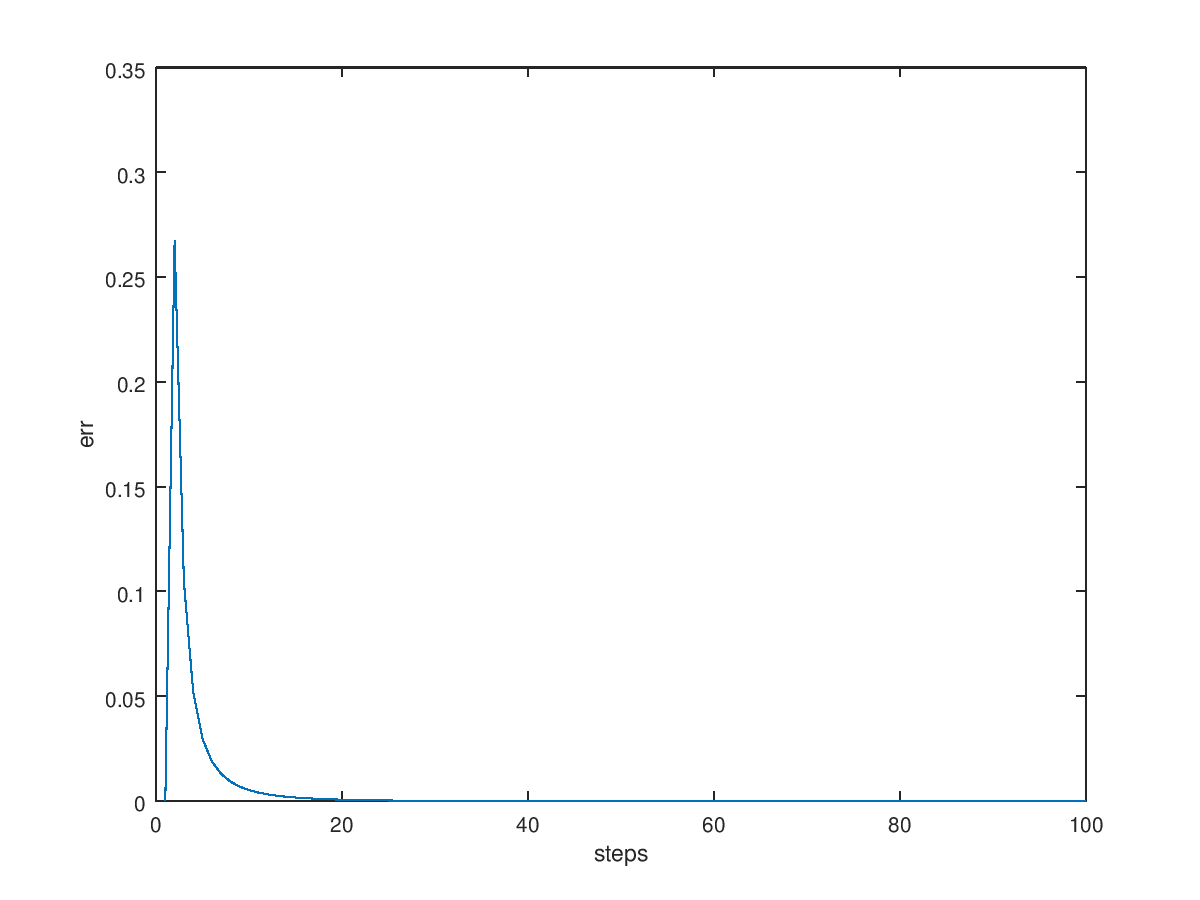
\includegraphics[scale=0.6]{figure/p1_done.png}
	\caption{Error converge to zero}
	\label{fig1}
\end{figure}

$$
A =
\begin{bmatrix}
	8.28151 &  4.78602 &  3.11495 &  9.72092 &  0.96063 &  8.03893 \\
   6.25617  &  9.31190 &  0.44826 &  6.97058 &  7.70458 &  8.94475 \\
   3.32950  &  3.06789 &  6.95169 &  2.94029 &  4.18702 &  2.11245 \\
   0.88935  &  2.30576 &  2.55318 &  6.62191 &  7.35451 &  0.82943
\end{bmatrix}
$$
$$
W * H =
\begin{bmatrix}
	8.28151 &  4.78602 &  3.11495 &  9.72092 &  0.96063 &  8.03893 \\
   6.25617  &  9.31190 &  0.44826 &  6.97058 &  7.70458 &  8.94475 \\
   3.32950  &  3.06789 &  6.95169 &  2.94029 &  4.18702 &  2.11245 \\
   0.88935  &  2.30576 &  2.55318 &  6.62191 &  7.35451 &  0.82943
\end{bmatrix}
$$
   
Because W and H must be non-negative, with some A, the error is not converge to zero.
\begin{figure}[htbp]
\centering
	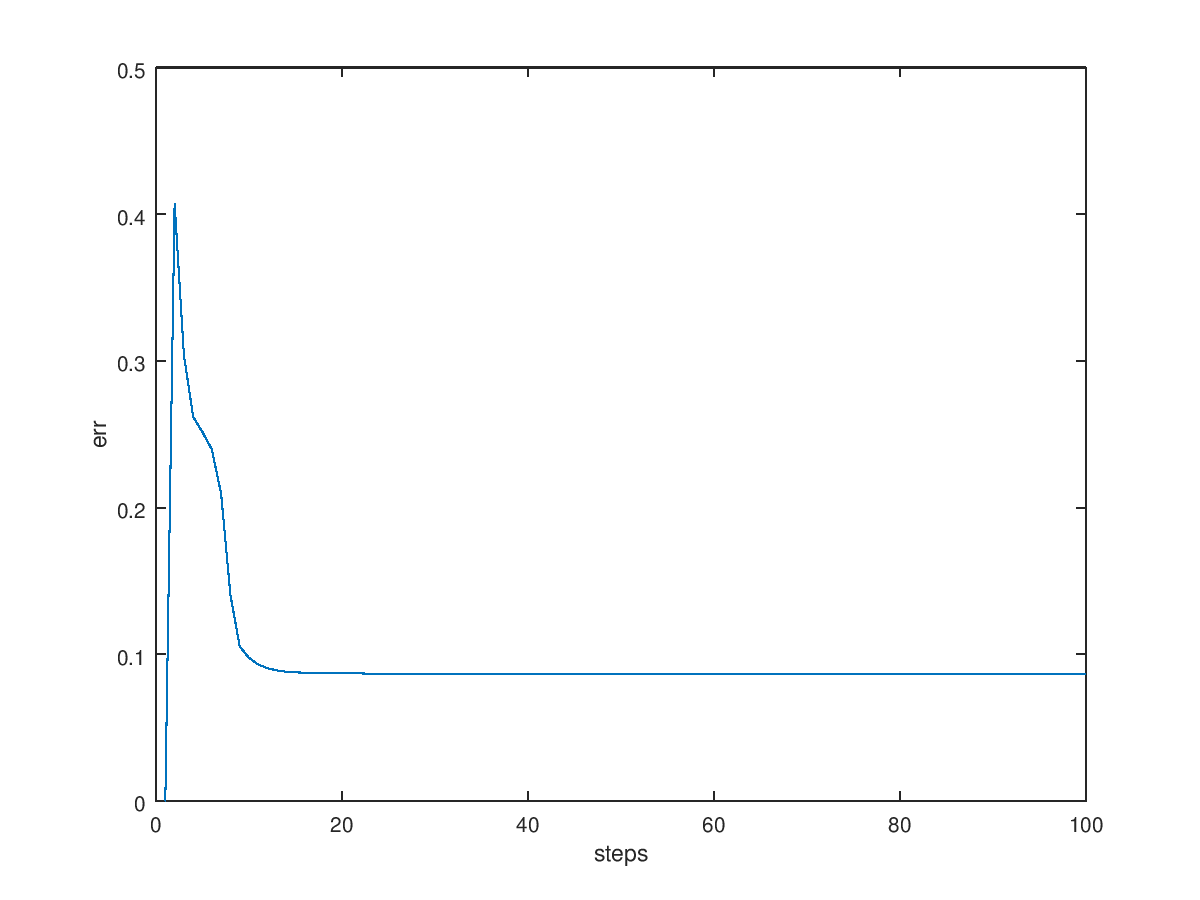
\includegraphics[scale=0.6]{figure/p1_err.png}
	\caption{Error not converge to zero}
	\label{fig2}
\end{figure}


$$
A =
\begin{bmatrix}
	8.94266 &  2.76995 &  0.62838 &  1.09185 &  0.39564 &  9.82682 \\
   4.41329  &  5.48933 &  9.45504 &  1.22046 &  3.40368 &  2.80803 \\ 
   1.64445  &  0.39538 &  7.17032 &  5.33515 &  5.52892 &  8.13614 \\
   6.54697  &  4.31847 &  0.27928 &  8.80909 &  0.56928 &  3.89232
\end{bmatrix}
$$
$$
W * H = 
\begin{bmatrix}
   8.39228 &  3.80541 &  0.62838 &  1.17900 &  1.25641 &  9.77508 \\
   4.80152 &  4.81932 &  9.45502 &  1.16976 &  3.79627 &  2.78443 \\
   2.03089 &  1.42680 &  7.17033 &  5.41319 &  4.92456 &  8.17246 \\
   6.83519 &  3.73378 &  0.27927 &  8.75588 &  0.98135 &  3.96163 
\end{bmatrix}
$$



\newpage
\section*{Problem 2}


\begin{lstlisting}[language = Matlab, numbers=left,   
  numberstyle=\tiny,keywordstyle=\color{blue!70},  
  commentstyle=\color{red!50!green!50!blue!50},frame=shadowbox,  
  rulesepcolor=\color{red!20!green!20!blue!20},basicstyle=\ttfamily,
  tabsize=2]
m = 1000;
n = 500;
k = 5;
d = 0.2;
lambda = 10;

U = rand(m,k);
V = rand(n,k);
I = find(rand(m,n) >= d);
A = U*V';
PA = A;
PA(I) = 0;

M = rand(m,k) * rand(n,k)';
err = zeros(100,1);
for j = 1:100
  % Take a step of the thresholded SVD iteration with threshold lambda.
  PAM = A - M;
  PAM(I) = 0;
  M = M + PAM;
  [U, S, V] = svd(M);
  S = max(S - eye(size(S)) .* lambda, zeros(size(S)));
  M = U * S * V';
  MM = M;
  MM(I) = 0;
  err(j) = norm(MM-PA)/norm(PA);
end
plot(err)
title('Error v.s. Iter-times');
xlabel('Iter-times');
ylabel('Error');
\end{lstlisting}

The result is:
\begin{figure}[htbp]
\centering
	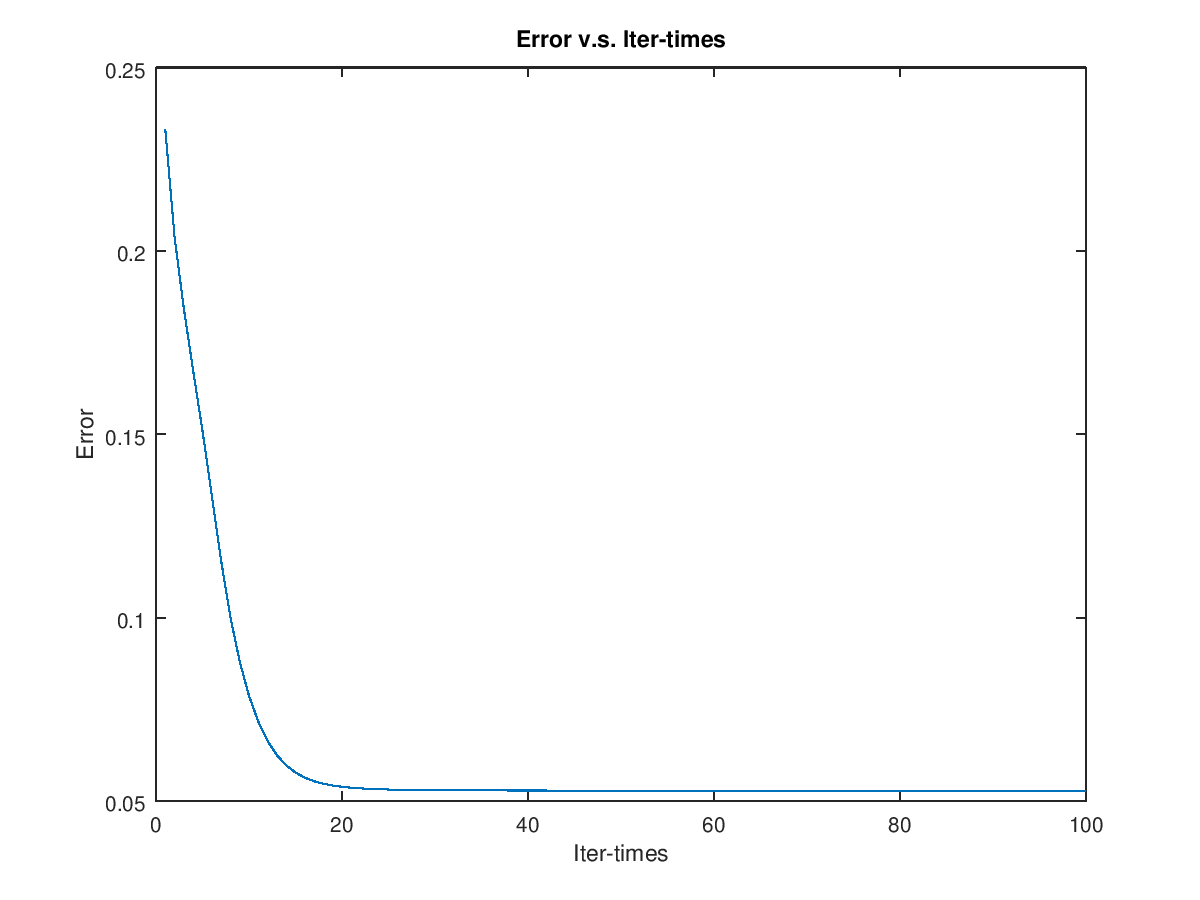
\includegraphics[scale=0.6]{figure/p2.png}
	\caption{SVDT}
	\label{fig3}
\end{figure}

The error is less than 0.1, which means it's a good approximation.

\section*{Problem 3}
My code is:
\begin{lstlisting}[language = Matlab, numbers=left,   
  numberstyle=\tiny,keywordstyle=\color{blue!70},  
  commentstyle=\color{red!50!green!50!blue!50},frame=shadowbox,  
  rulesepcolor=\color{red!20!green!20!blue!20},basicstyle=\ttfamily,
  tabsize=2]
m = 1000;
n = 500;
k = 5;
d = 0.2;
lambda = 10;

U = rand(m,k);
V = rand(n,k);
tmp = rand(m,n);
exist = tmp < d;
I = find(tmp >= d);

A = U*V';
PA = A;
PA(I) = 0;

X = rand(m,k);
Y = rand(n,k);
M = X * Y';
M(I) = 0;
err = zeros(100,1);
for l = 1:100
  err(l) = norm(M - PA)/norm(PA);
  for i = 1:m
	  loca = find(exist(i, :) ~= 0);
	  y = Y(loca,:);
	  a = A(i,:)';
	  a = a(loca,:);
	  X(i, :) = ((y' * y + lambda * eye(k,k)) \ (y' * a))';
  end
  for j = 1:n
	  loca = find(exist(:, j) ~= 0);
	  x = X(loca,:);
	  a = A(:,j);
	  a = a(loca,:);
	  Y(j, :) = ((x' * x + lambda * eye(k,k)) \ (x' * a))';
  end
  M = X*Y';
  M(I) = 0;
end
plot(err)
title('Error v.s. Iter-times');
xlabel('Iter-times');
ylabel('Error');
\end{lstlisting}

The result is:
\begin{figure}[htbp]
\centering
	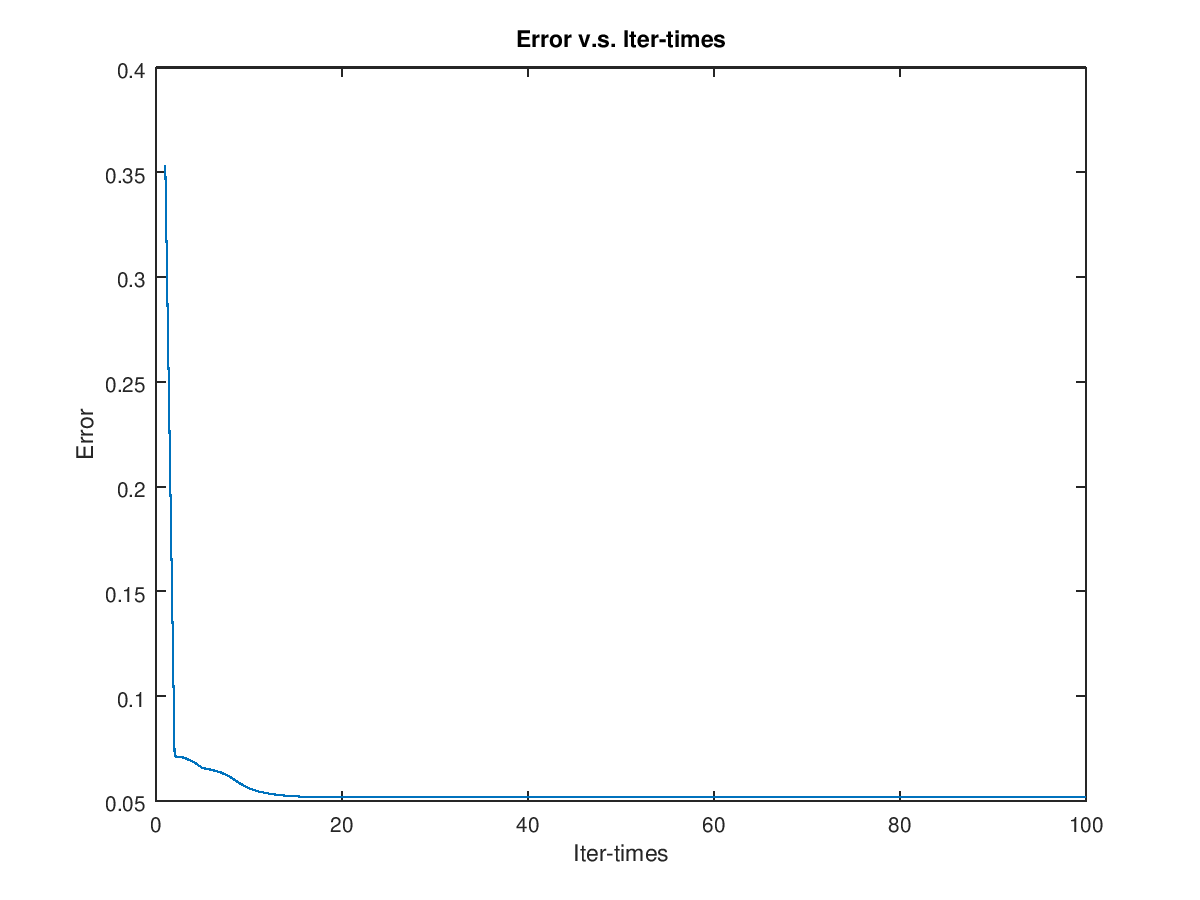
\includegraphics[scale=0.6]{figure/p3.png}
	\caption{ALS}
	\label{fig4}
\end{figure}

\end{document}
